WebMGA 3.0 is a visualisation tool for molecular simulation outputs which refines on previous versions by \textcite{Battistini_2021,webmga_2}. It provides a more modern, maintainable, and accessible alternative to the older QMGA tool by \textcite{gabriel2008molecular}. The program is available as a web app at REMOVED\footnote{Text removed for submission since URL contains author name. Visible at \cite{webmga_3_app}.}, with source code at REMOVED\footnote{Text removed for submission since URL contains author name. Visible at \cite{webmga_3_github}.}. Development utilised JavaScript with the React\cite{react} framework and three.js\cite{three} 3D graphics library. This project aimed to fix existing issues in WebMGA and further enhance the existing feature set. Most effort was focused on implementing additional molecule geometries and optimising existing geometries, improving visualisation for the axes and director (defined in \cref{director_explain}), visualising periodic repetitions of a configuration (defined in \cref{pbc_explain}), and implementing a distance based variable Level of Detail optimisation.

Since the project aimed to work on an existing program, development was structured to begin with bug fixing, followed by implementing previously identified missing features, and finally extending the feature set based on user feedback.

This report provides a background summary explaining the requirements and terminology for molecular simulation rendering (\cref{context_section}), descriptions for the changes required and made for WebMGA 3.0 (\cref{req_section,imp_section}), and quantitative summaries for performance improvements and qualitative analysis of rendered systems (\cref{analysis_sec}). Finally, achievements are summarised and the project successes evaluated (\cref{conc_eval_sec}).

\begin{figure}
  \begin{center}
    \begin{subfigure}{0.4\textwidth}
      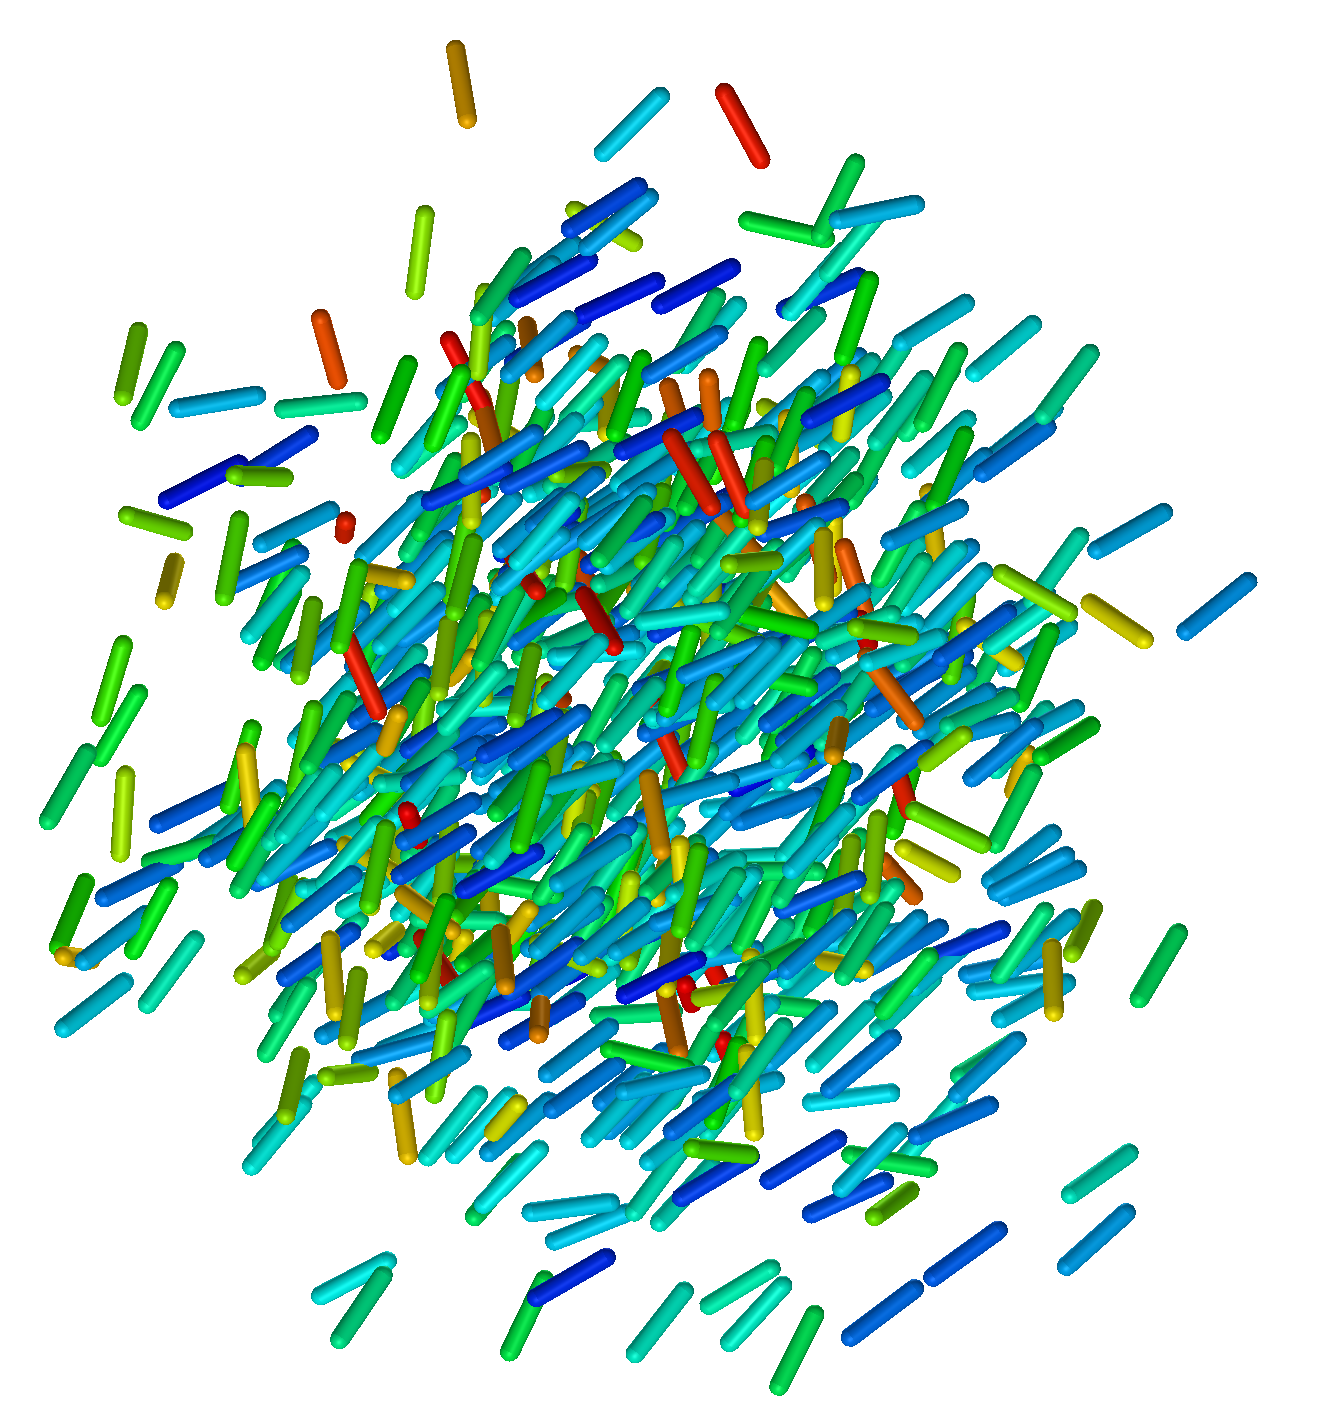
\includegraphics[width=\textwidth]{assets/images/configs/nematic}
      \caption{Unfolded SC4 Nematic.}
      \label{sc4_fig}
    \end{subfigure}
    \begin{subfigure}{0.4\textwidth}
      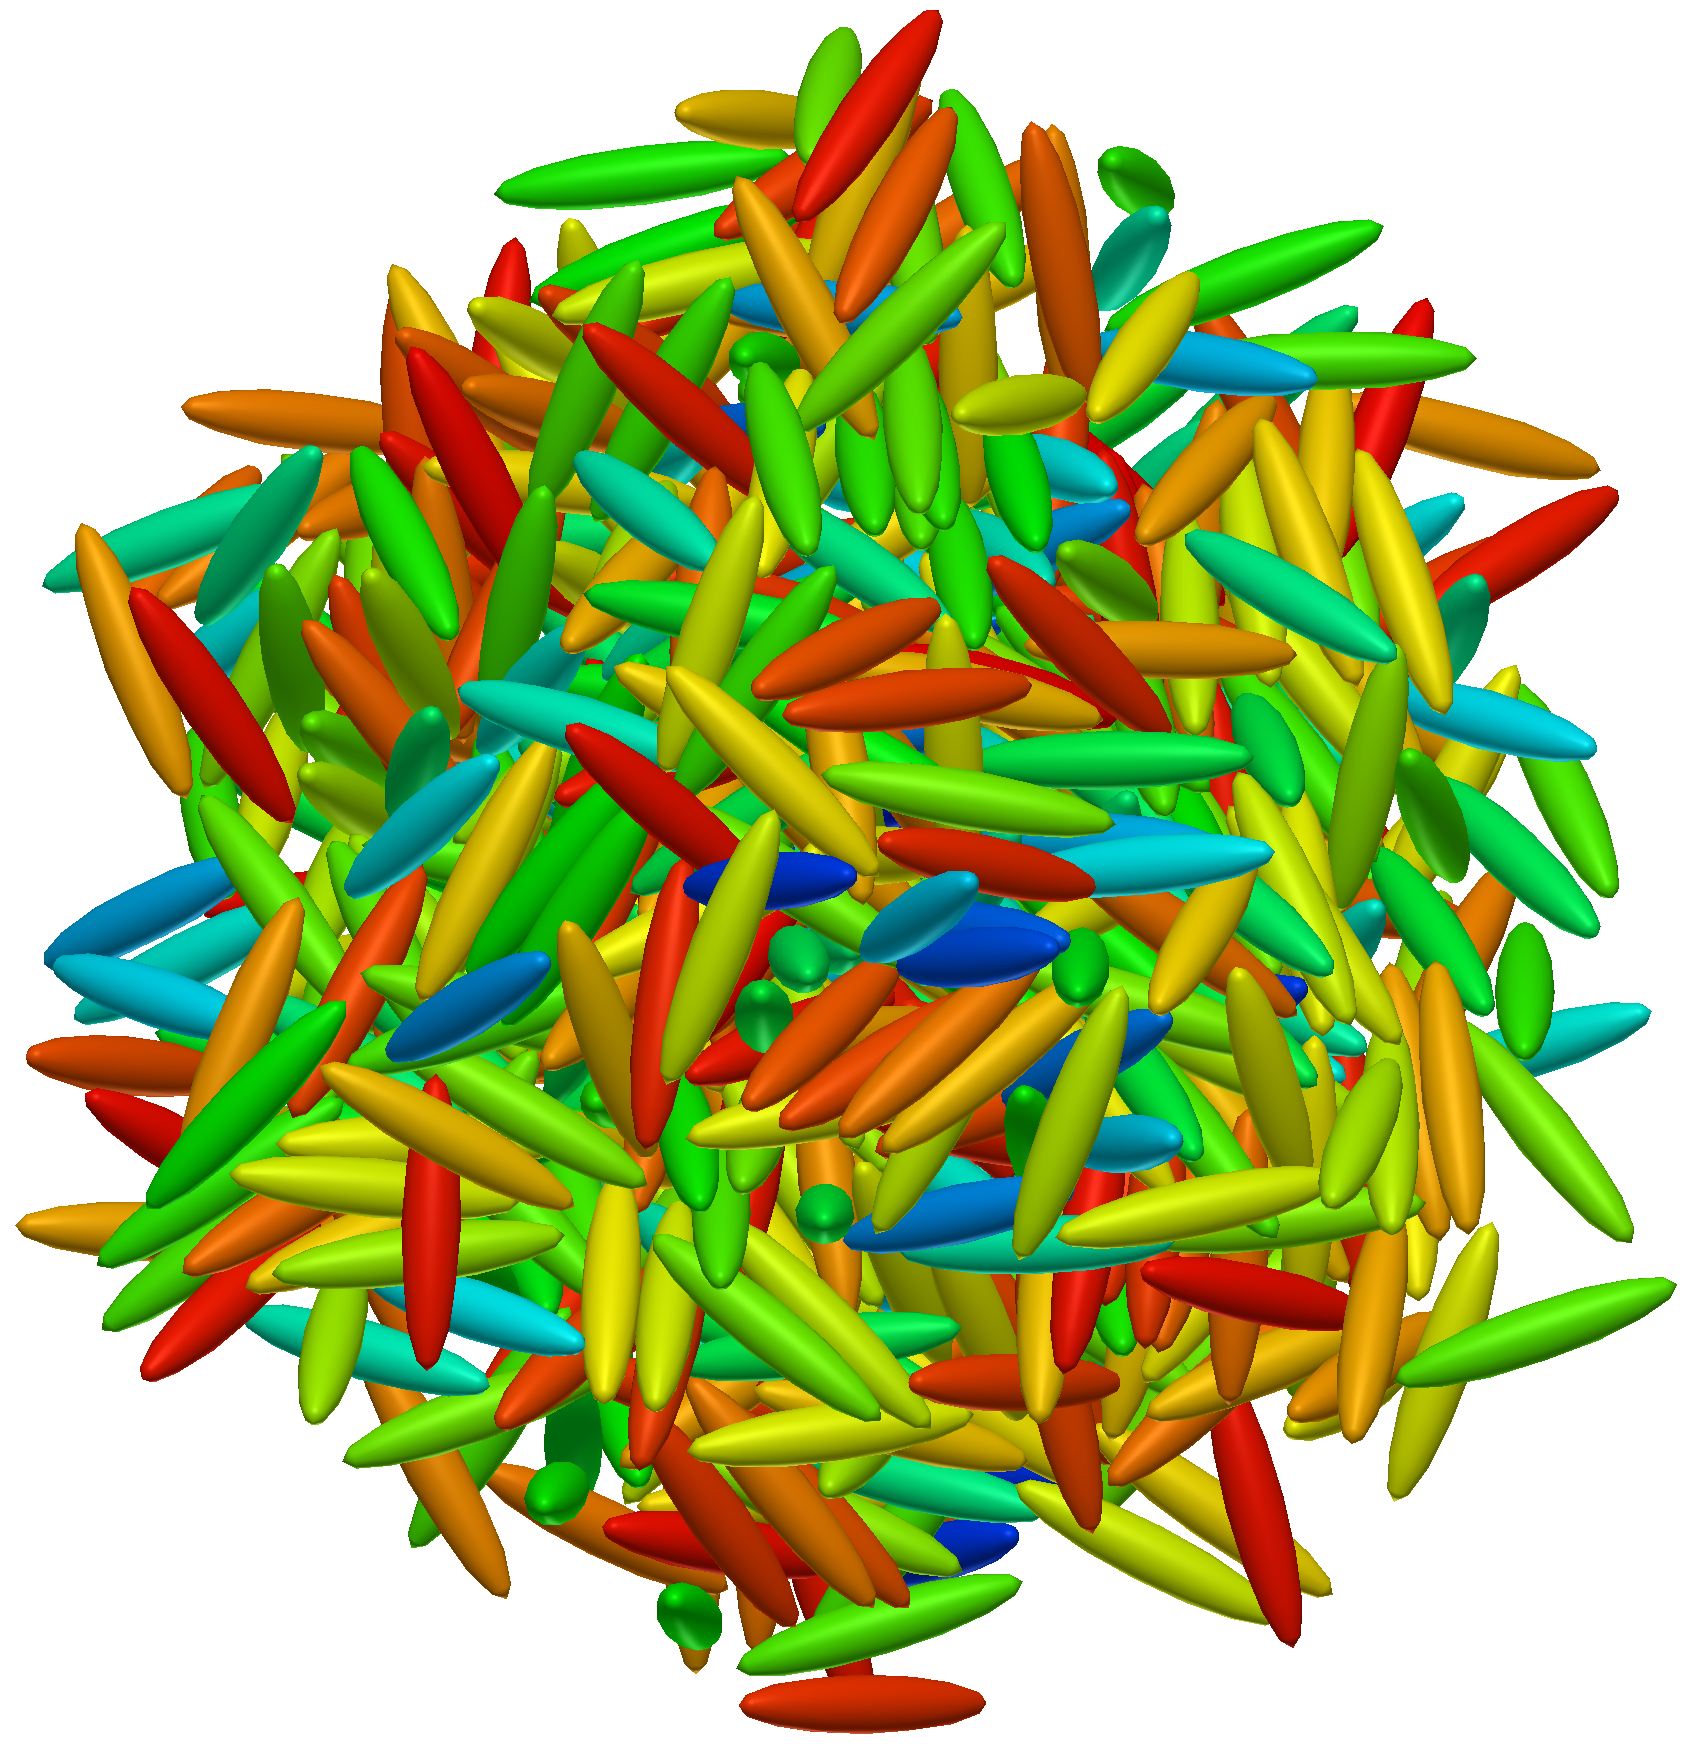
\includegraphics[width=\textwidth]{assets/images/configs/iso}
      \caption{E5 Isotropic.}
    \end{subfigure}
    \begin{subfigure}{0.4\textwidth}
      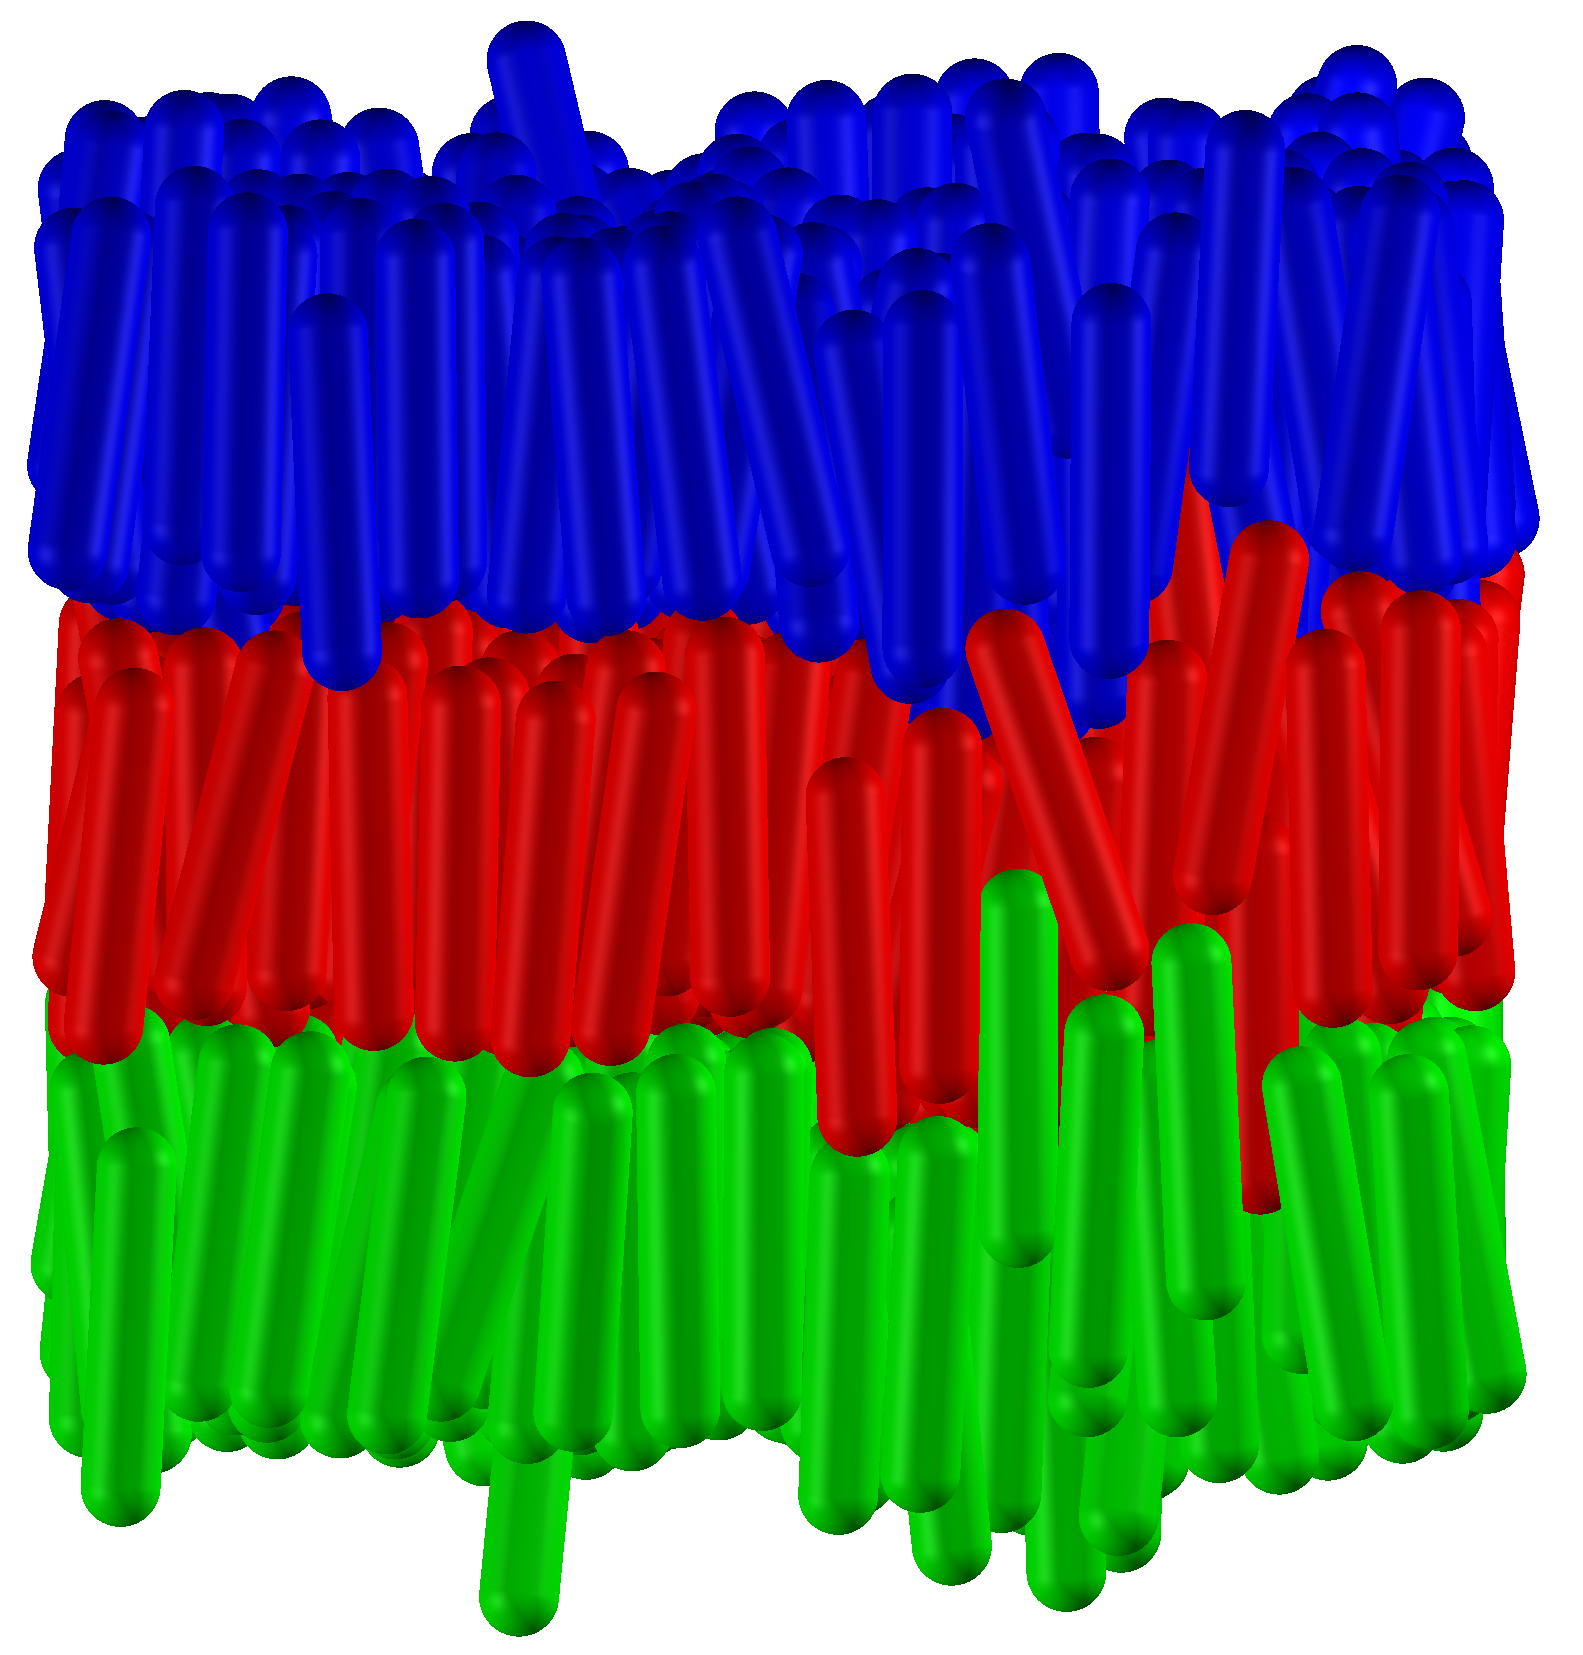
\includegraphics[width=\textwidth]{assets/images/configs/smectic}
      \caption{SC4 Smectic.}
    \end{subfigure}
    \begin{subfigure}{0.4\textwidth}
      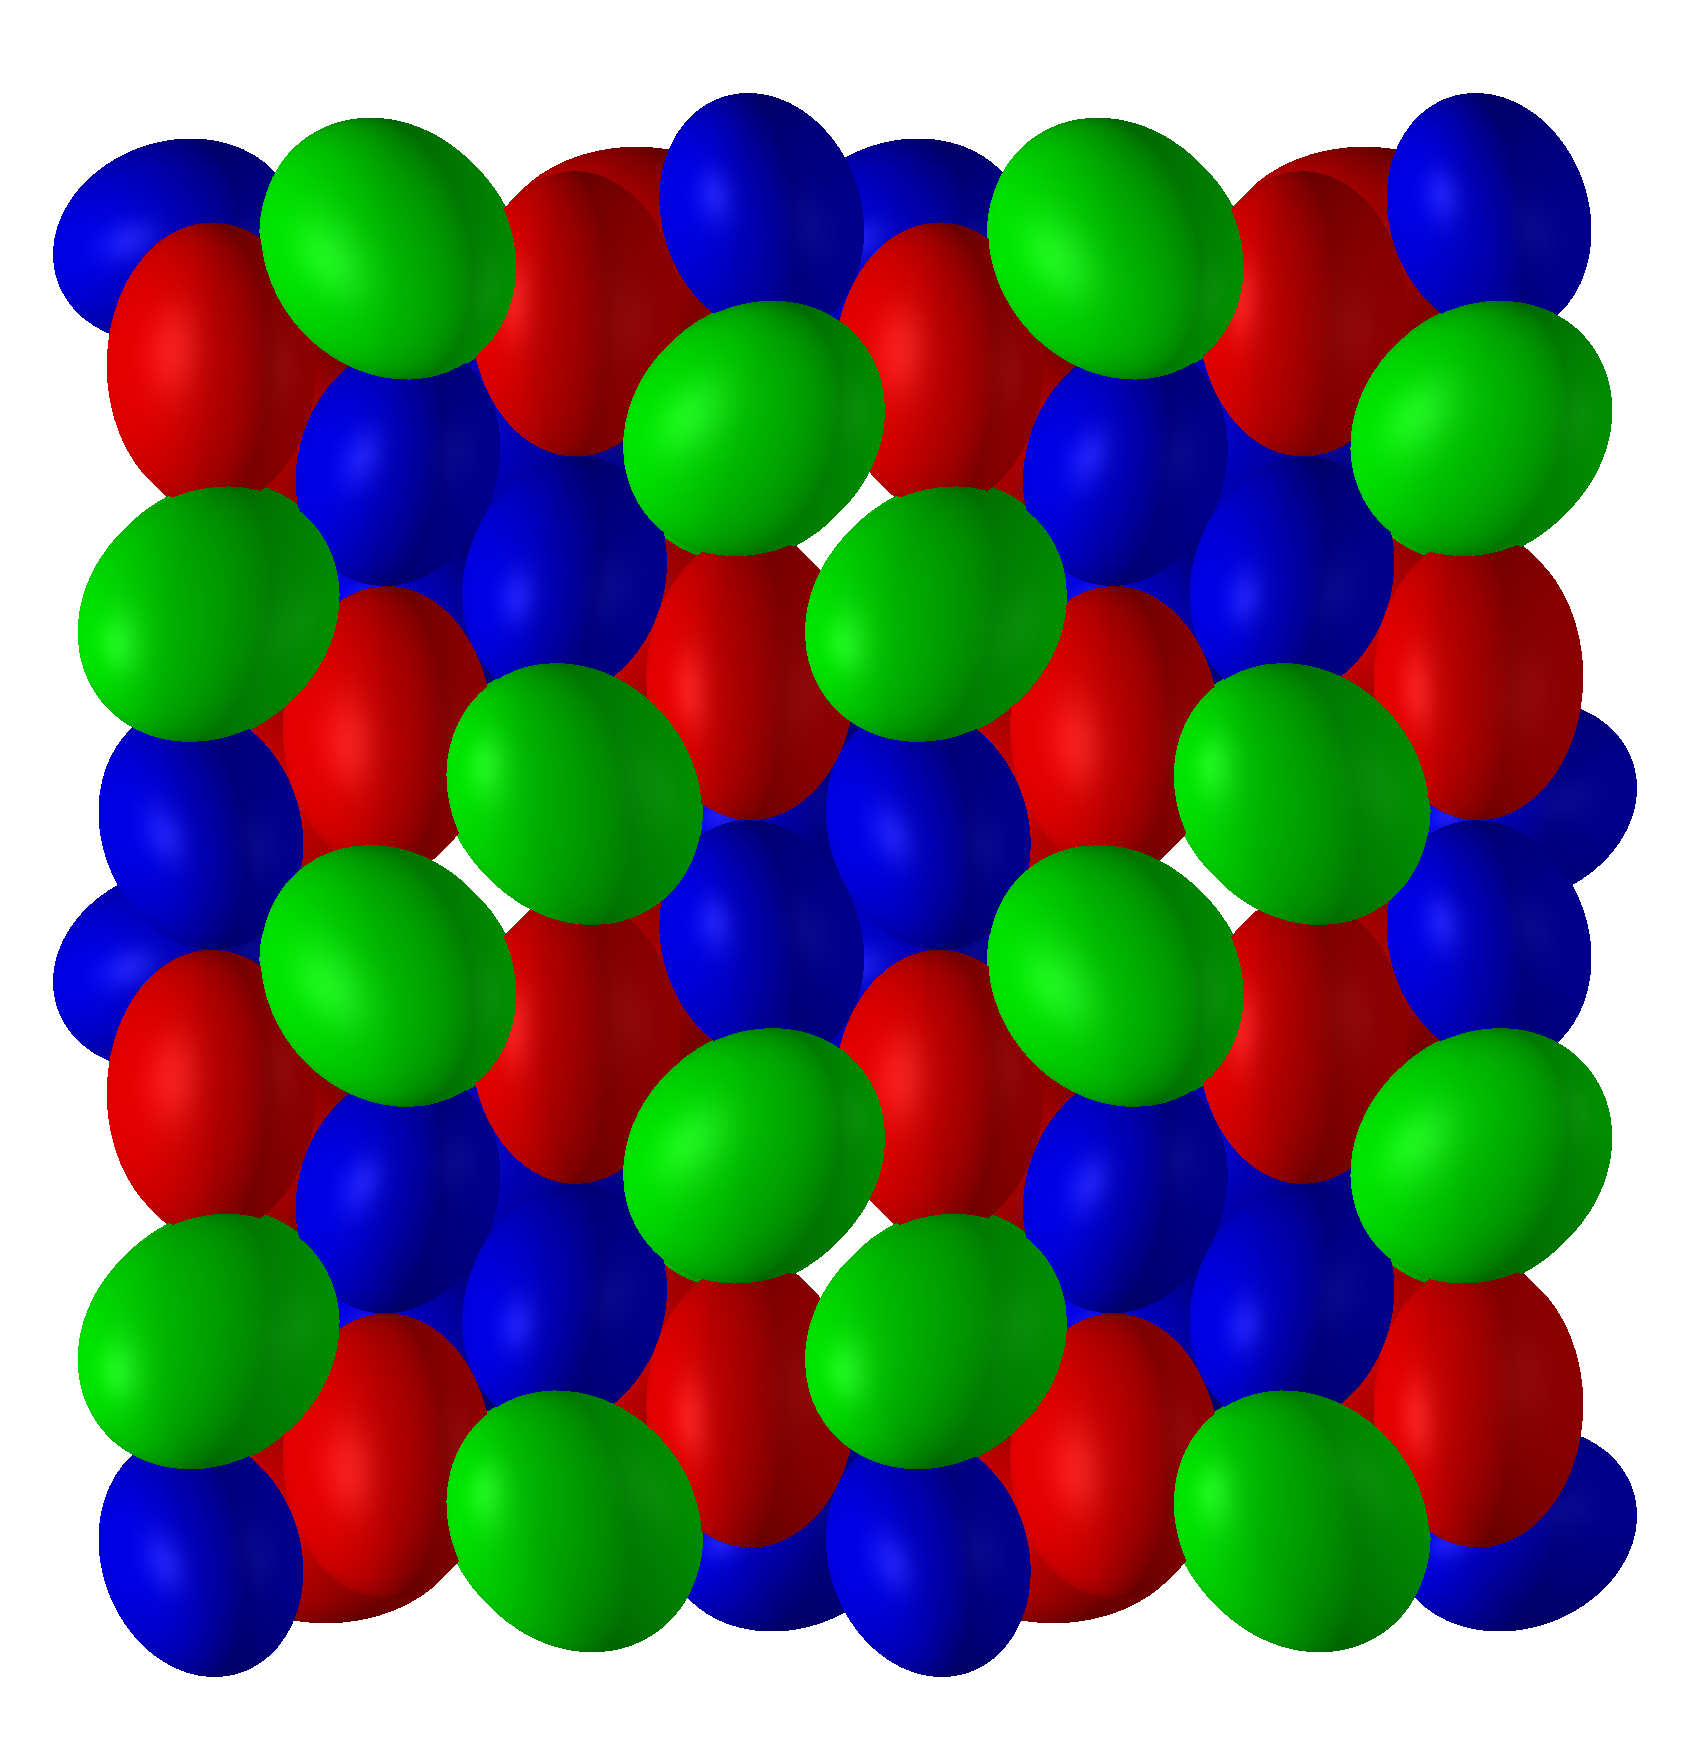
\includegraphics[width=\textwidth]{assets/images/configs/biaxial}
      \caption{Biaxial Crystal.}
    \end{subfigure}
    \begin{subfigure}{0.4\textwidth}
      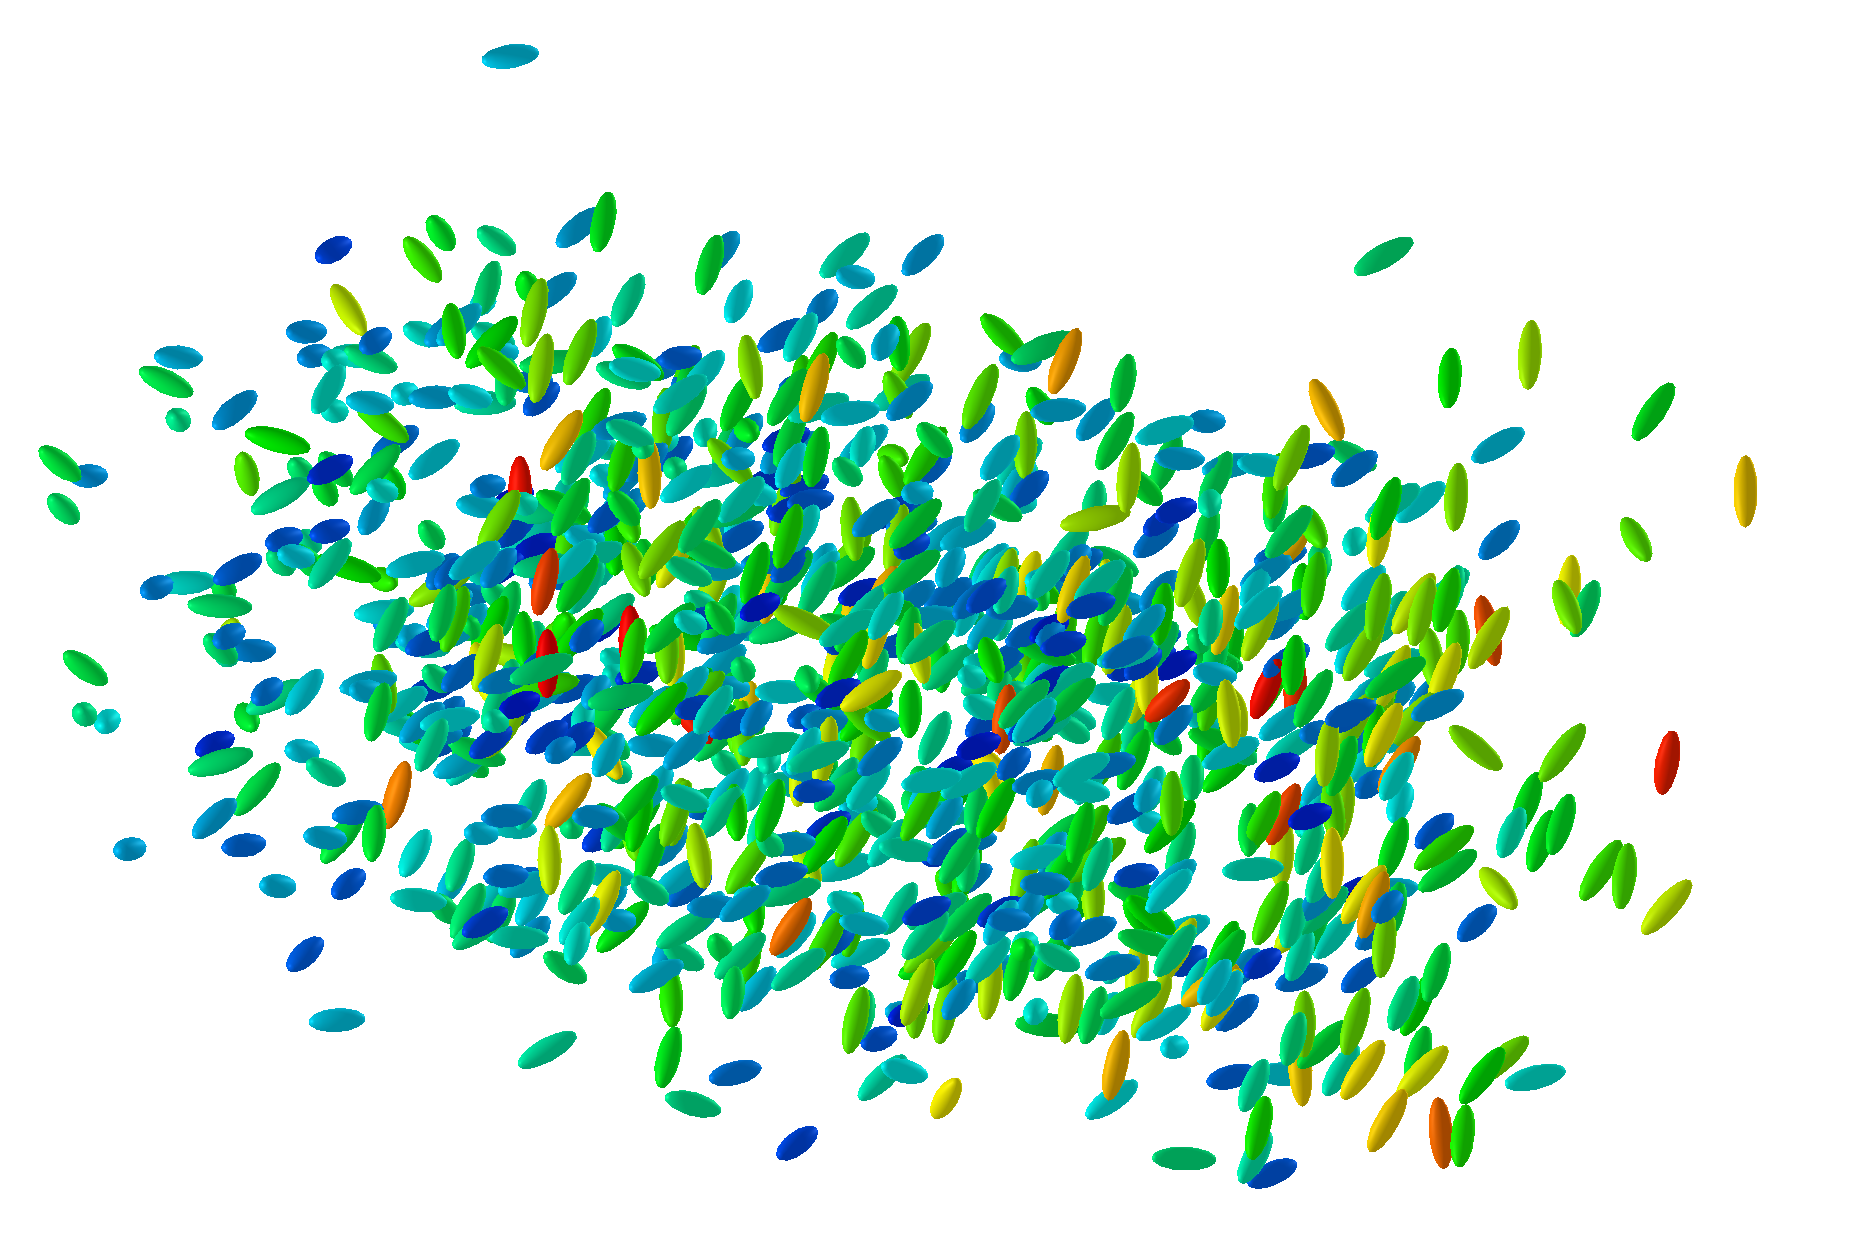
\includegraphics[width=\textwidth]{assets/images/configs/chiral}
      \caption{Unfolded E3 Chiral Nematic.}
    \end{subfigure}
    \begin{subfigure}{0.4\textwidth}
      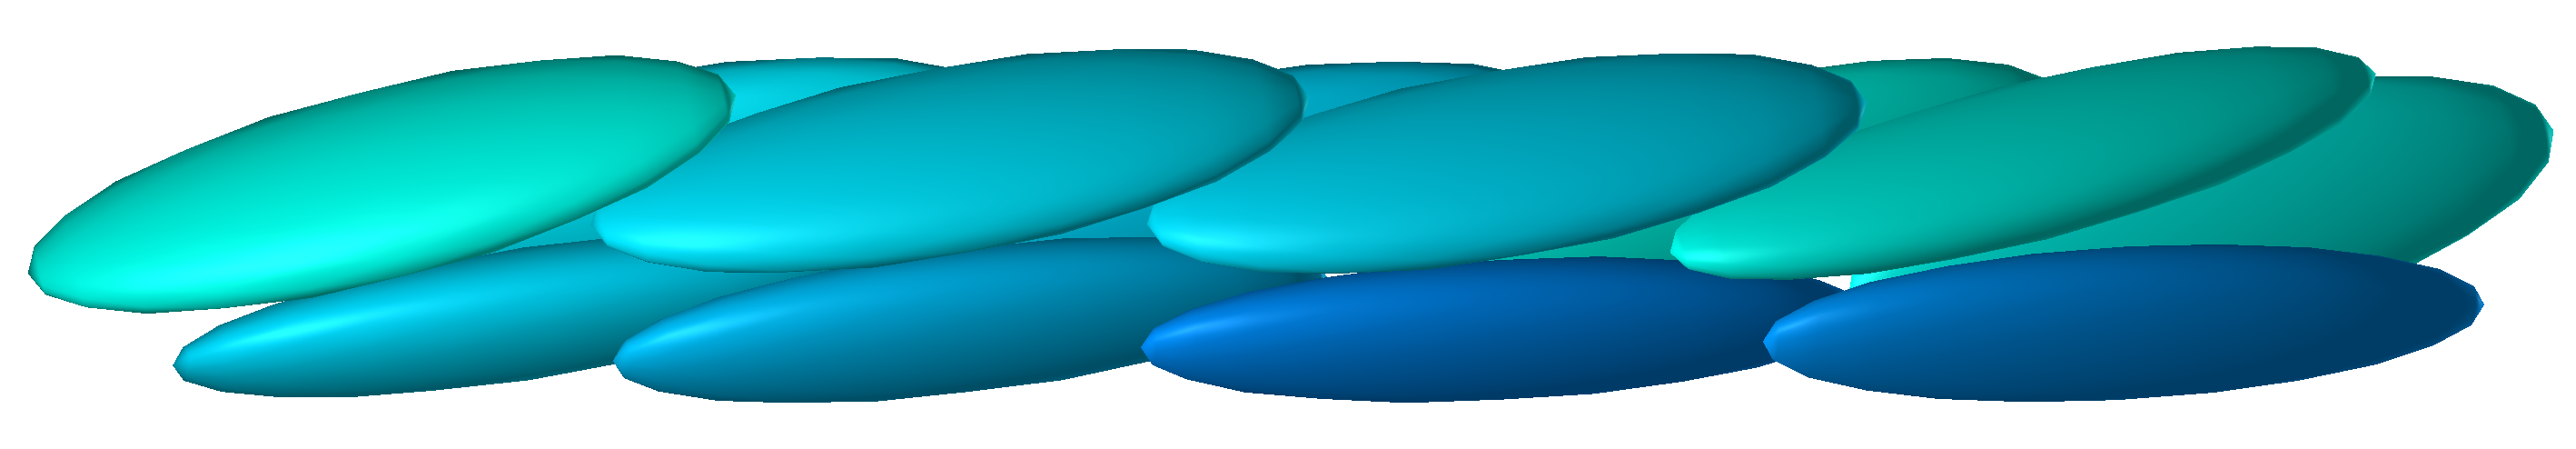
\includegraphics[width=\textwidth]{assets/images/configs/hbc}
      \caption{HBC (In Cylinder).}
    \end{subfigure}
  \end{center}
  \caption{Various configurations generated using WebMGA 3.0.}
  \label{fig:assorted_configs}
\end{figure}
